\chapter{Estado del arte}

El concepto MTD se empieza a popularizar de forma teórica en informática (ya que no es exclusiva de esta) hace unos 10 años. Se han realizado investigaciones aplicándolo a diferentes ámbitos de la informática, donde con el paso de las investigaciones se ha ido creando una clasificación de las diferentes técnicas de MTD \cite{big-state-of-art}.
\begin{figure}[h]
    \centering
    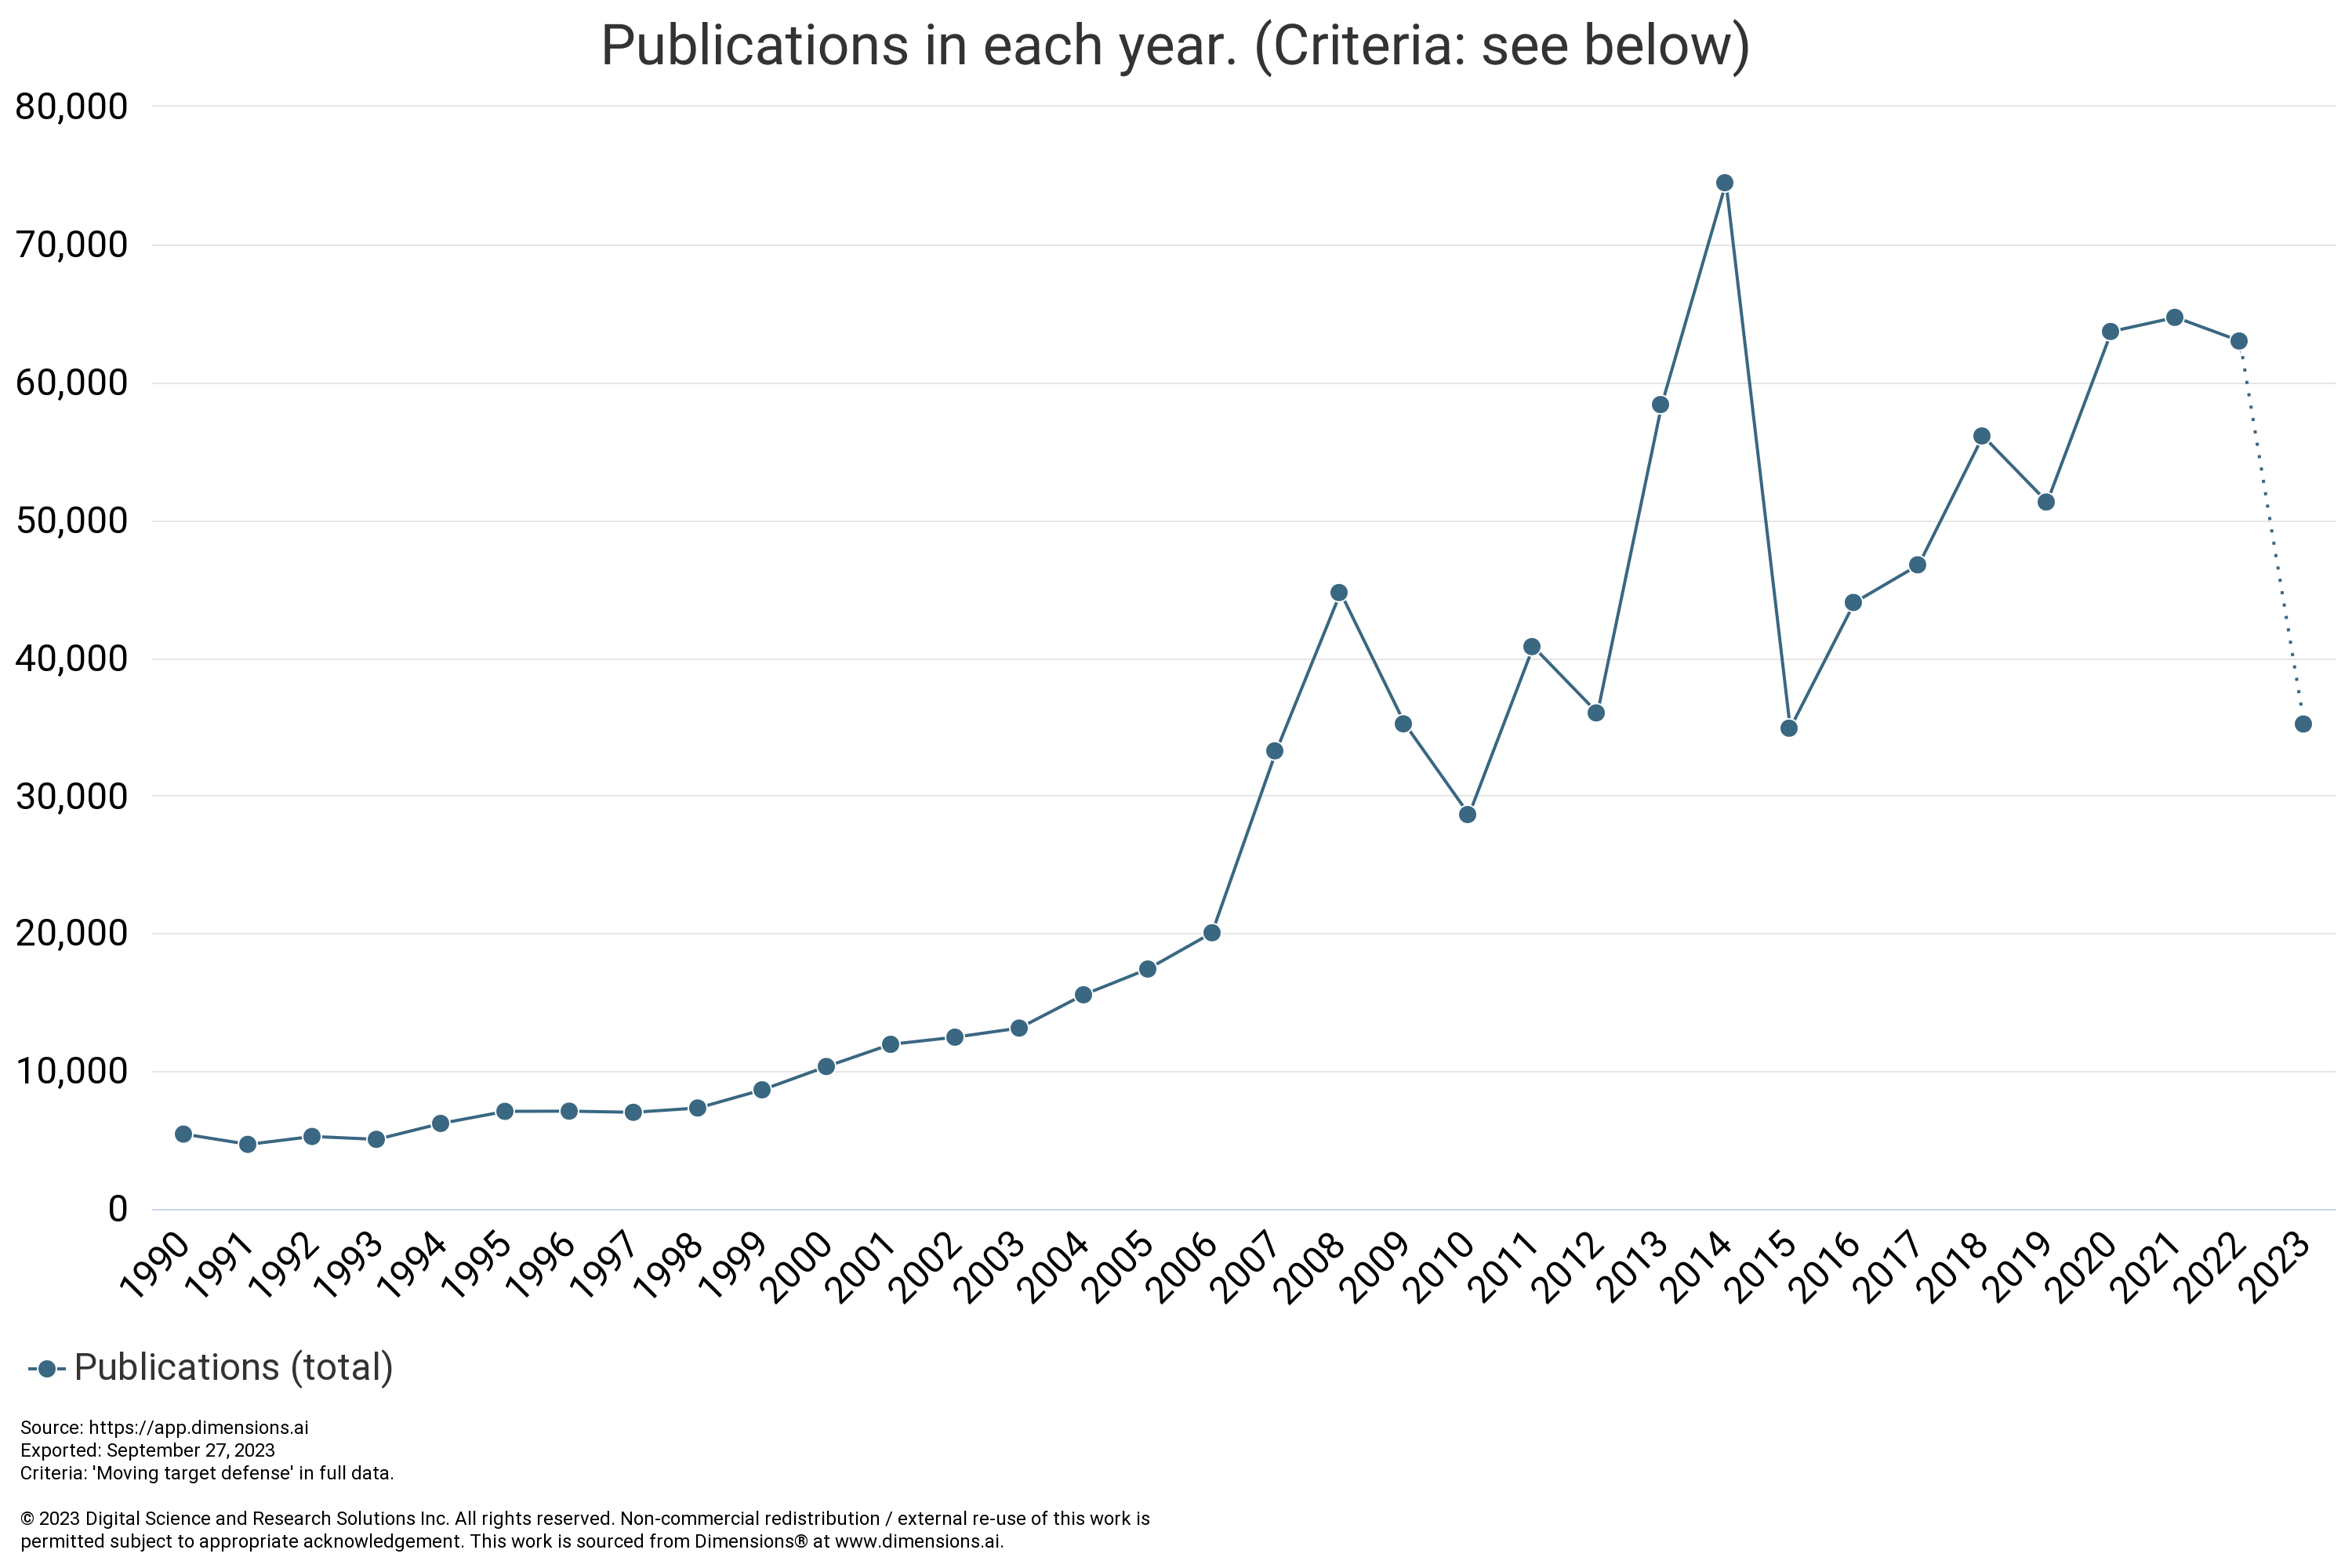
\includegraphics[width=\linewidth]{./imagenes/busquedasMTD.png}
    \caption{Investigaciones sobre MTD a lo largo del tiempo}
\end{figure}

A continuación vamos a hacer una revisión sobre los aspectos más importantes de los MTD, como son la clasificación y limitaciones. Además haremos un repaso sobre las implementaciones que se han realizado sobre servidores web, ya que es el objetivo de este trabajo.

\section{Clasificación}
Cuando queremos implementar un MTD, necesitamos elegir el componente más viable o donde necesitamos más protección.

\textbf{Qué mover}: debería ser un componente o atributo que habilite un vector de ataque. Por ejemplo, pueden ser una IP \cite{MTD-SDN+decoy}\cite{MTD-ipshuffling+honeypots}\cite{MTD-POC-empresa}, servidor web \cite{MTD-DARE}\cite{MTD-MORE+DARE+Java}, sistema operativo \cite{MTD-MORE+DARE+Java}, direcciones de memoria \cite{MTD-ASR}, base de datos \cite{MTD-arab}, WAF \cite{MTD-WAF}, VM \cite{MTD-POC-empresa}\cite{MTD-DARE}\cite{SCIT-base}, etc.

\textbf{Cómo moverlo}: una vez se ha seleccionado el componente, hay que determinar como cambiarlo, para esto hay tres opciones diferentes:
\begin{itemize}
    \item Mezcla: se cambia un componente por otro, los ejemplos de componentes incluyen direcciones IP de un servidor o las variables de entorno de un sistema.
    \item Diversidad: tiene componentes diferentes que realizan la misma tarea, por ejemplo, en vez de varios servidores Apache como servidores web, tiene un Apache y dos Nginx.
    \item Redundancia: tener componentes repetidos para asegurar que, si uno falla o es comprometido, otros pueden tomar su lugar o mitigar el impacto del ataque. 
\end{itemize}

\begin{figure}[h]
    \centering
    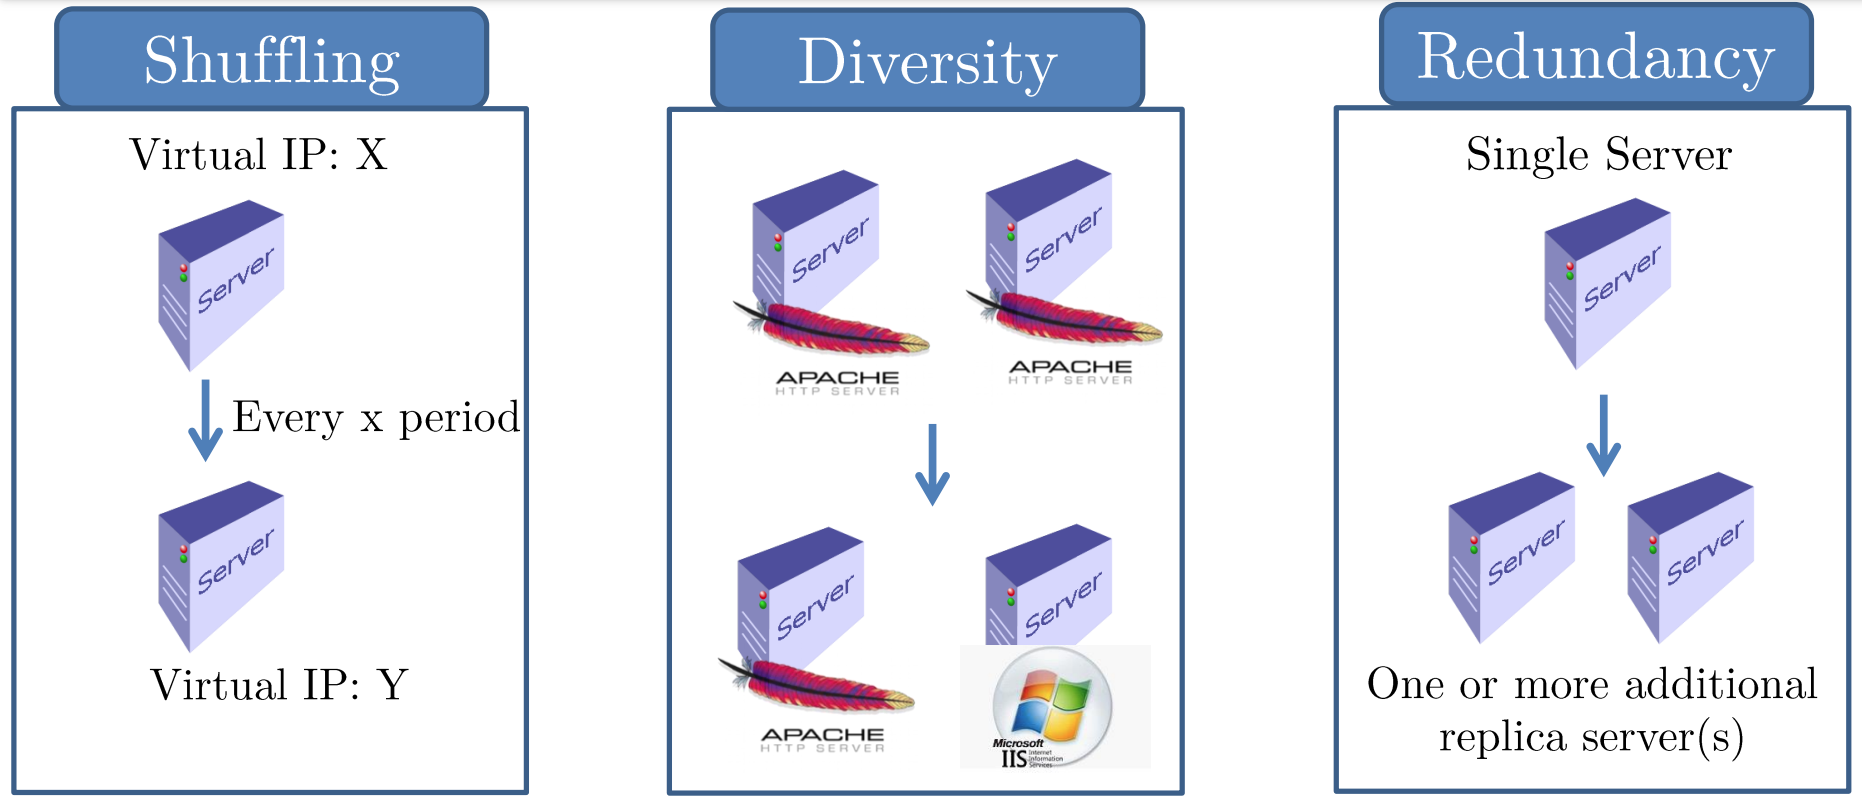
\includegraphics[width=\linewidth]{./imagenes/tiposmovimientos.png}
    \caption{Formas de mover un componente}
\end{figure}

\textbf{Cuándo moverlo}: una vez que se ha seleccionado el componente y la forma de moverlo, hay que determinar cuando moverlo. Hay dos opciones:
\begin{itemize}
    \item Por tiempo (proactivo): se mueve el componente de forma periódica, independientemente de si se ha detectado un ataque o no. El periodo no tiene por qué ser fijo, puede ser aleatorio o entre un rango de tiempo.
    \item Por evento (reactivo): se mueve el componente cuando se detecta un ataque o un fallo en el sistema, la forma de detectarlo puede ser machine learning\cite{MTD-ML}, uso de IPS\cite{Design-Generic-Intrusion-Tolerant-Architecture}, un WAF \cite{MTD-WAF}, etc.
\end{itemize}

Esta clasificación no es excluyente, es decir se pueden combinar diferentes opciones. Por ejemplo, se pueden combinar las dos opciones de cuando moverlo (creando una opción híbrida) con todas las opciones de como moverlo. La mayoría de veces una implementación combina varios de estas \cite{MTD-MORE+DARE+Java}\cite{MTD-DARE}\cite{MTD-arab}, aunque que exista esta posibilidad no quiere decir que se deban de mezclar todas las opciones posibles, ya que podrían dar configuraciones menos seguras o eficientes que al utilizar menos opciones \cite{MTD-comparativa-gorda}.

\section{Servidores web}
Los MTD basados en servidores web no son una de las principales líneas de investigación, ya que son más difíciles de adaptar a un entorno de producción, no hay consenso sobre ellos y no han demostrado tener resultados tan eficaces como otras líneas (SDN o \textit{IP shuffling}). Aun así, se han realizado varias implementaciones sobre estos, nos centraremos en aquellos que rotan los servidores que se utilizan, comenzando por el DARE (\textit{Dynamic Application Rotation Environment for Moving Target Defense}) este se basa en la estrategia utilizada por el MORE (\textit{Multiple Operating System Rotational Environment MTD})\cite{MORE}, la cual consiste en ir cambiando la máquina que recibe el tráfico mediante IP. DARE lo implementa en los puertos, esta consiste en rotar un servidor Nginx\cite{nginx} con uno Apache\cite{apache}, los cuales están en la misma máquina, para servir una página web estática. Esto lo logran utilizando un script como servicio el cual cambia la entrada de Iptables\cite{iptables} para apuntar a un puerto u otro.

El problema de DARE es que al actualizar el firewall, se perdía mucha disponibilidad al reiniciar el servicio, por lo que a partir de esta, surge \textit{DARE IMproved} (DIM). Este utiliza la misma estrategia que DARE, pero utiliza un script en Python el cual altera Iptables, pero no reinicia el servicio. Esto es posible, ya que si una regla está definida correctamente en Iptables, no es necesario reiniciarlo para que entre en funcionamiento, llevando la disponibilidad hasta el 98\%. Otra mejora que hace DIM respecto a DARE, es que redirige el tráfico a los servidores mediante el \textit{loopback}, lo que permite que los servidores no sean accesibles desde fuera de la máquina. Con estas mejoras se consiguieron aumentar la disponibilidad, rendimiento y la seguridad.

A pesar de las mejoras llevadas a cabo, la disponibilidad sigue sin ser suficiente, algunos sitios web deben tener una disponibilidad del 99.99\% para cumplir con el acuerdo de nivel de servicio (SLA)\cite{SLA}, al modificar Iptables, los paquetes que estaban siendo procesados por el servidor son descartados automáticamente. Por lo que surge \textit{Mutable Asymmetric web Server Security} (MASS), el cual está basado en las implementaciones anteriores, con las siguientes mejoras:
\begin{itemize}
    \item Utiliza Firewalld\cite{firewalld}: es una alternativa a Iptables, la cual tampoco reinicia el servicio. Además, este puede controlar el flujo de paquetes, por lo que mientras que un servidor está siendo cambiado, los paquetes son almacenados en una cola para ser enviados al acabar el cambio.
    \item Uso de contenedores: ahora cada servidor está en un contenedor diferente, lo que aumenta el aislamiento, ya que si anteriormente si un servidor era comprometido, toda la máquina lo era también.
    \item Reencarnación de contenedores: esta técnica consiste en que una vez que un contenedor es cambiado por el otro contenedor, en vez de mantenerlo o comprobar si ha sido comprometido, es destruido directamente, para volver a crear un contenedor nuevo a partir de una imagen base.
\end{itemize}

Alejándose de la línea anterior, otra implementación es la de Philip Tibom y Max Buck\cite{MTD-gotemburgo}, en la que utilizan nodos de Kubernetes\cite{kubernetes} para implementar el MTD. Esta configuración consigue un 100\% de disponibilidad. Utiliza \textit{VM shufflig}, cambiando los nodos entre diferentes ubicaciones físicas y su IP. Está preparado para utilizar distintas imágenes de Docker en diferentes nodos.

El SCIT (\textit{Self Cleansing Intrusion Tolerance})\cite{SCIT-base} es otra tecnología vinculada a los servidores web. Esta estrategia se basa en la reencarnación de un componente, similar a lo que realiza MASS. En 2011, se publicó un estudio\cite{SCIT-cloud}, que compartía estructura con el trabajo de Philip Tibom y Max Buck; sin embargo, en este caso se implementaba el SCIT. Es notable mencionar que, pese a los 11 años transcurridos desde ambas investigaciones, no se ha liberado ningún software de código abierto que emulase dicha implementación.


\section{Limitaciones}
A pesar de las diferentes investigaciones e implementaciones que existen, muchas tienen en común algunas malas prácticas y clichés que se repiten, dando lugar a un análisis erróneo de los resultados. Estas prácticas son:
\begin{itemize}
    \item Pruebas de explotación pobres: la evaluación de la defensa se suele centrar en la fase de reconocimiento, para después utilizar un único \textit{exploit} en la explotación por componente, esto hace las pruebas más fáciles, pero no da una visión realista de la seguridad, ya que utiliza un único vector de ataque, el cual no varía el tiempo que se tarda en explotar la vulnerabilidad.
    \item MTD por eventos o híbridos dejados atrás: las investigaciones e implementaciones se suelen centrar en MTD proactivos, ya que una de las características que se le atribuye a los MTD es que son inseguros por defecto. Por lo que las líneas principales de investigación se centran en mantener el rendimiento, ofuscar el reconocimiento y reducir el tiempo que un componente es vulnerable. Si bien es cierto que los MTD proactivos pueden cumplir con estos objetivos y la mayor parte de la investigación debería seguir esa línea, dejar de lado los eventos se aleja de una solución realista, por un ejemplo tan sencillo como que en un MTD con diversidad o redundancia de servidores, uno de ellos esté caído y se le siga mandando tráfico.
    \item Aumento de la superficie de ataque: en determinados MTD proactivos la rotación de un componente puede aumentar las brechas de seguridad\cite{MTD-critica}, este es un problema intrínseco a esta tecnología, que se suele pasar por alto en la mayoría de investigaciones. Se podrían dar las siguientes situaciones como ejemplo:
    \begin{enumerate}
        \item Tenemos un componente seguro y otro inseguro: si rotamos entre ellos cada cierto tiempo, el sistema será vulnerable la mitad del tiempo. La solución realista sería dejar de cambiar al vulnerable al detectar el ataque.
        \item Si tenemos dos componentes seguros: el sistema no será vulnerable nunca, si los componentes son diferentes uno rendirá mejor que el otro. La solución realista sería mantener el componente que mejor rendimiento tenga, y si los componentes son iguales, no haría falta rotarlos, una configuración estática sería más óptima.
        \item Tenemos dos componentes inseguros: el sistema será vulnerable siempre. La solución realista sería realizar cambios constantemente hasta parchear las vulnerabilidades, que serían dos en vez de una.
    \end{enumerate}
    Como hemos dicho antes estos ejemplos no aplican a todas las tecnologías MTD, pero son uno de los problemas de raíz de esta tecnología.
    \item Atribuir la seguridad al cambio erróneamente: es decir realizamos una rotación entre diferentes componentes, pero el cambio no es gracias a utilizar un componente diferente. Un ejemplo, tenemos una vulnerabilidad que causa una denegación de servicio (DoS) en un servidor, esta tarda 30 s en empezar a funcionar y 60 s en dejar el servidor caído. Si realizamos cambios cada 15 s entre el servidor vulnerable y uno seguro (reiniciando el servidor al cambiarlo), el servidor nunca estará caído, pero no es gracias a la rotación, sino al reinicio. Si realizáramos la rotación entre dos servidores vulnerables, el servidor tampoco estaría caído, ya que el tiempo de explotación es mayor que el del cambio de componente.
    \item Falta de código \textit{opensource}: apenas hay código abierto sobre los MTD, esto hace que sea difícil replicar los resultados de las investigaciones, ya que no se puede saber si se ha implementado correctamente o no. Además de retrasar la investigación al tener que reinventar la rueda y no poder realizar comparativas entre soluciones.
\end{itemize}

\section{Analogías}

Alexander Bajic y Georg T. Becker listaron una serie de analogías\cite{MTD-critica} con los ejemplos anteriores:
\begin{itemize}
    \item El combate aéreo y bandada de pájaros: en un combate aéreo, un piloto debe hacer maniobras impredecibles para no ser un blanco fácil. Esta situación ilustra cómo las tácticas de seguridad de TI actuales son estáticas, como esperar en un búnker. Algunas empresas usan la analogía de una bandada de pájaros, donde cada ave se mueve constantemente, dificultando que un depredador ataque a una específica.
    \item La caza del ciervo: Un ciervo en movimiento puede eludir a un cazador que lo persigue. Sin embargo, si el cazador espera en un punto, dicho movimiento es lo que lo pone en peligro. Es vital considerar no solo cómo este beneficia a la defensa, sino también cómo podría beneficiar al atacante. Un ejemplo de esto es el aumento de superficie de ataque que se mencionó anteriormente.
    \item El trilero: una bola se esconde bajo uno de los tres cubiletes que se mueven rápidamente. Sin embargo, este juego suele ser un engaño, ya que el operador manipula sigilosamente la bola. Aunque el movimiento de los cubiletes puede no ser el factor de seguridad en la MTD, otros aspectos de la defensa sí lo son.
\end{itemize}

\begin{figure}[h]
    \centering
    \begin{minipage}{.3\textwidth}
        \centering
        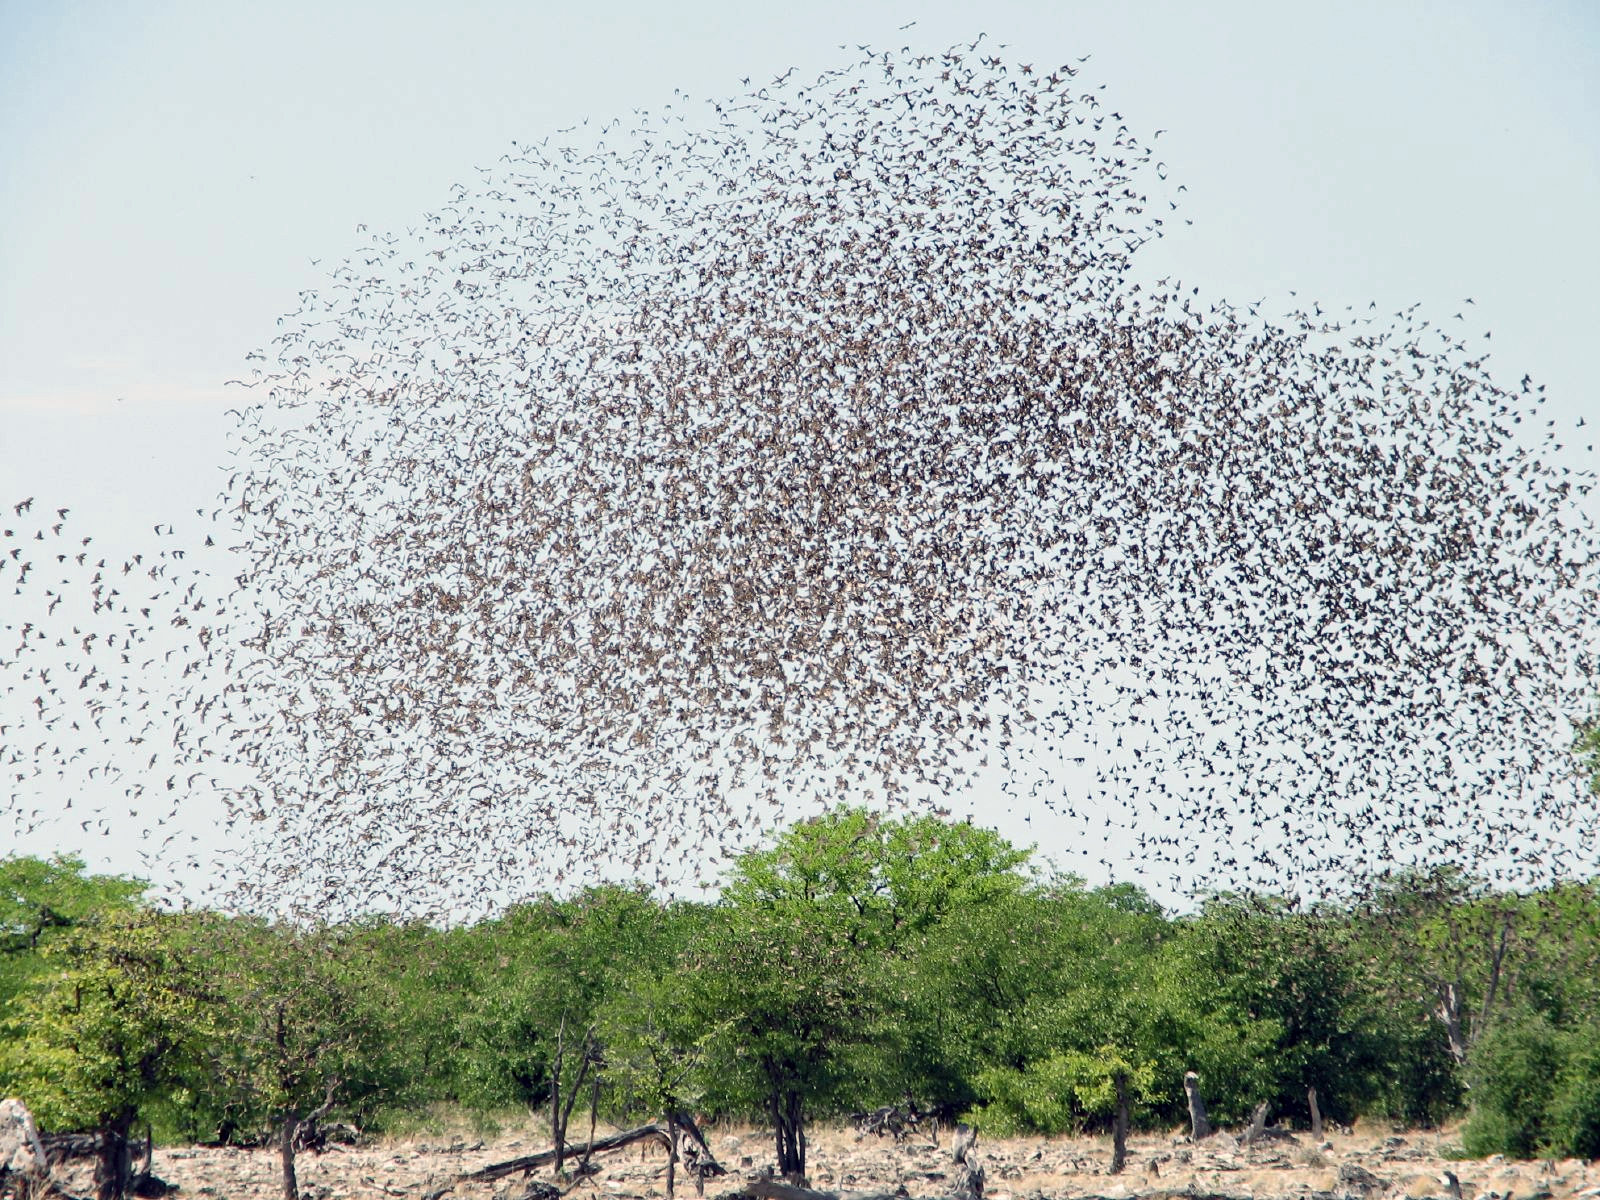
\includegraphics[width=\linewidth]{./imagenes/bandada.jpg}
        \caption{Bandada de pájaros}
    \end{minipage}
    \hfill
    \begin{minipage}{.3\textwidth}
        \centering
        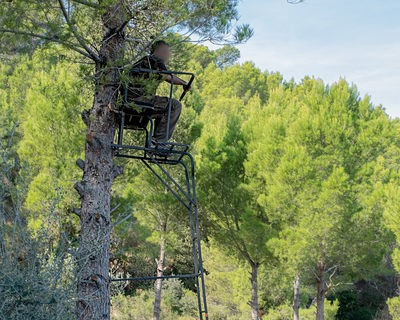
\includegraphics[width=\linewidth]{./imagenes/caza.jpg}
        \caption{Cazador esperando que el ciervo se ponga a tiro}
    \end{minipage}
    \hfill
    \begin{minipage}{.3\textwidth}
        \centering
        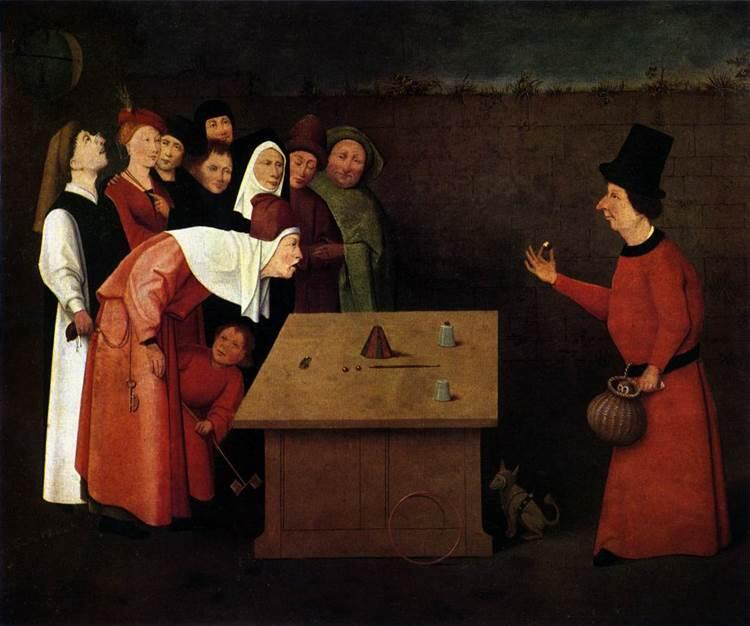
\includegraphics[width=\linewidth]{./imagenes/trilero.jpg}
        \caption{Trilero}
    \end{minipage}
\end{figure}
